\section{Information to test the new models}
\label{sect:model}
We would like to quote our reconstruction efficiencies in a way that is as model independent as possible. For this
we carefully define the acceptance, and provide details about the selection efficiency within that acceptance. In
this way, anybody can use their favorite Monte Carlo generator of new physics, define an acceptance at the hard
scatter level (e.g. status = 3 in Pythia 6), and correctly estimate the efficiency for this new physics model to within
50\% or so (the so-called ``outreach'' program).

The event selection efficiency is a combination of
\begin{itemize}
\item the kinematic requirements on leptons and taus;
\item the lepton identification and isolation efficiency;
\item the efficiency of the \MPT requirement;
%\item the efficiency of the b-tagged jets veto;
%\item the efficiency of the extra lepton veto;
\item the efficiency of the invariant mass requirement;
%\item the efficiency of the \mindphifour requirement;
\item the efficiency of the \mttwo requirement;
\item the efficiency of the \mt requirements.
\end{itemize}


Efficiencies are provided against the kinematic properties (e.g., \pt) of visible $\tau$ objects at generator level. The visible $\tau$ (\visTau), if it decays leptonically, is defined as the 4-vector of the lepton. In hadronic decays, the difference between the 4-vector of $\tau$ and its neutrino is attributed to the visible $\tau$. %It is, hereafter, referred to as \visTau.
The visible $\tau$ objects are required to pass the offline kinematic selections ($\eta$ and \pt requirements). The \genMET variable is defined as the magnitude of the negative vector sum of \visTau pairs in the transverse plane. The 4-vector of the \visTau objects and \genMET are used to calculate the transverse mass (\mt) of the \visTau objects and also the generated \mttwo. All efficiencies are derived in the 
``TChipChimSlepSnu'' sample, which is a chargino pair production sample. The chargino mass goes from 120 to 500 \GeV and the neutralino mass goes from 
1 to 500 \GeV.
Table \ref{tbl:EffTauLep}
\begin{table}[!htb]
\begin{center}
\caption{Efficiencies to select a lepton or \Tau in different channels. $\Tau^1$ and $\Tau^2$ stand for leading and next-to-leading \Tau in the \tauTau channel.}
\begin{tabular}{|c|c|c|c|c|c|}
\hline\hline
\pt(\visTau) (\GeV)       & e for $e\Tau$ & $\mu$ for $\mu\Tau$  & \Tau for $\ell\Tau$    &  $\Tau^1$ for \tauTau & $\Tau^2$ for \tauTau\\
\hline\hline
%0-10                      &    0.15       &    0.01              &         0.001          &       0.0             & 0.52 \\\hline
%10-20                     &    0.14       &    0.72              &         0.004          &       0.0             & 0.54\\\hline
20-30                     &    0.27       &    0.80              &         0.12           &       0.0             & 0.56\\\hline
30-40                     &    0.68       &    0.86              &         0.20           &       0.0             & 0.55\\\hline
40-60                     &    0.75       &    0.87              &         0.21           &       0.02            & 0.61\\\hline
60-80                     &    0.80       &    0.89              &         0.23           &       0.08            & 0.69\\\hline
80-120                    &    0.83       &    0.90              &         0.25           &       0.12            & 0.70\\\hline
120-160                   &    0.85       &    0.91              &         0.26           &       0.15            & 0.70\\\hline
160-200                   &    0.87       &    0.91              &         0.27           &       0.16            & 0.71\\\hline
$>$ 200                   &    0.89       &    0.92              &         0.28           &       0.17            & 0.71\\\hline
\hline
\end{tabular}
\label{tbl:EffTauLep}
\end{center}
\end{table}
shows the efficiencies of selecting a lepton or \Tau for different channels versus the transverse momentum (\pt) of the \visTau. The efficiencies include 
the scale factors and efficiencies of object identification and isolation and trigger also.
The values are calculated in the events that pass  \genMET $>$ 30 \GeV.
Table \ref{tbl:EffMet}
\begin{table}[!htb]
\begin{center}
\caption{Efficiency to pass the \MPT  requirement in different channels versus the \genMET.}
\begin{tabular}{|c|c|}
\hline\hline
\genMET  (\GeV)        & all channels\\
\hline\hline
0-10                   &    0.52 \\\hline
10-20                  &    0.58 \\\hline
20-30                  &    0.68 \\\hline
30-40                  &    0.79 \\\hline
40-50                  &    0.87 \\\hline
50-60                  &    0.93 \\\hline
60-70                  &    0.95 \\\hline
70-80                  &    0.97 \\\hline
80-90                  &    0.98 \\\hline
90-100                 &    0.98 \\\hline
100-120                &    0.99 \\\hline
120-140                &    0.99 \\\hline
140-160                &    0.99 \\\hline
160-200                &    1.0  \\\hline
$>$ 200                &    1.0  \\\hline
\hline
\end{tabular}
\label{tbl:EffMet}
\end{center}
\end{table}
shows the efficiency in different channels to pass the \MPT $>$ 30 \GeV as a function of the \genMET. 
%The mass of the system of the selected pair is used to parametrize 
%the efficiency to pass the cuts on the reconstructed invariant mass. 
The following efficiencies are calculated in the generated events that pass  \genMET $>$ 30 \GeV.
Table \ref{tbl:EffMass}
\begin{table}[!htb]
\begin{center}
\caption{Efficiency to pass the invariant mass requirements in different channels versus the generated mass.}
\begin{tabular}{|c|c|c|}
\hline\hline
generated mass (\GeV)  & $\ell\Tau$  &  \tauTau \\
\hline\hline
0-5                  &    0.00     &   0.00   \\\hline
5-10                 &    0.10     &   0.25   \\\hline
10-15                &    0.20     &   0.60  \\\hline
15-20                &    0.97     &   0.90  \\\hline
20-25                &    1.00     &   0.94   \\\hline
25-30                &    1.00     &   0.98   \\\hline
30-35                &    1.00     &   1.00   \\\hline
35-40                &    0.99     &   1.00   \\\hline
40-45                &    0.84     &   0.99   \\\hline
45-50                &    0.16     &   0.95   \\\hline
50-55                &    0.04     &   0.68   \\\hline
55-60                &    0.02     &   0.18   \\\hline
60-65                &    0.01     &   0.06   \\\hline
65-70                &    0.04     &   0.03   \\\hline
70-75                &    0.22     &   0.05   \\\hline
75-80                &    0.78     &   0.15   \\\hline
80-85                &    0.91     &   0.41   \\\hline
85-90                &    0.95     &   0.79   \\\hline
90-95                &    0.97     &   0.93   \\\hline
95-100               &    0.98     &   0.96   \\\hline
100-105              &    1.00     &   0.98   \\\hline
105-110              &    1.00     &   0.99   \\\hline
110-115              &    1.00     &   0.99   \\\hline
$>$ 115              &    1.00     &   1.00   \\\hline
\hline
\end{tabular}
\label{tbl:EffMass}
\end{center}
\end{table}
shows the efficiency in different channels to pass the requirement of the reconstructed invariant mass versus the invariant mass of  
\visTau pair (generated mass). The requirements
on the invariant mass of the reconstructed pair are ($>$ 15 \GeV) and ($<$ 45 or $>$ 75 \GeV) for the $\ell\Tau$ channels 
and ($<$ 55 or $>$ 85 \GeV) for the \tauTau channel. 
The efficiency to pass the (\mttwo $>$ 90 \GeV) requirement in $\ell\Tau$ and \tauTau \binone is shown in Table \ref{tbl:EffMT2}. 
\begin{table}[!htb]
\begin{center}
\caption{Efficiency to pass the  \mttwo $>$ 90 \GeV requirement in different channels versus the generated \mttwo.}
\begin{tabular}{|c|c|c|}
\hline\hline
generated \mttwo (\GeV)    & $\ell\Tau$  &  \tauTau \binone \\
\hline\hline
0-20                     &    0.00     &   0.00  \\\hline
20-40                    &    0.002    &   0.01  \\\hline
40-50                    &    0.01     &   0.02  \\\hline
50-60                    &    0.02     &   0.04  \\\hline
60-70                    &    0.05     &   0.08  \\\hline
70-80                    &    0.13     &   0.19  \\\hline
80-90                    &    0.34     &   0.45  \\\hline
90-100                   &    0.65     &   0.73  \\\hline
100-110                  &    0.82     &   0.88  \\\hline
110-120                  &    0.90     &   0.94  \\\hline
120-130                  &    0.93     &   0.97  \\\hline
130-140                  &    0.95     &   0.98  \\\hline
140-160                  &    0.96     &   0.99  \\\hline
160-180                  &    0.97     &   0.99  \\\hline
180-200                  &    0.97     &   1.00  \\\hline
$>$ 200                  &    0.97     &   1.00  \\\hline
\hline
\end{tabular}
\label{tbl:EffMT2}
\end{center}
\end{table}
Table \ref{tbl:EffTauMT}
\begin{table}[!htb]
\begin{center}
\caption{Efficiency to pass the  \tauMT requirement in $\ell\Tau$ channels versus the generated \tauMT.}
\begin{tabular}{|c|c|}
\hline\hline
generated \tauMT (\GeV)  & $\ell\Tau$ \\
\hline\hline
%0-50                     &   0.35   \\\hline
%50-100                   &   0.1   \\\hline
100-125                  &   0.01   \\\hline
125-150                  &   0.03   \\\hline
150-170                  &   0.09   \\\hline
170-190                  &   0.25   \\\hline
190-200                  &   0.52   \\\hline
200-210                  &   0.66   \\\hline
210-230                  &   0.82   \\\hline
230-250                  &   0.91   \\\hline
250-275                  &   0.94   \\\hline
275-300                  &   0.97   \\\hline
$>$ 300                  &   1.00   \\\hline
\hline
\end{tabular}
\label{tbl:EffTauMT}
\end{center}
\end{table}
shows the efficiency in the $\ell\Tau$ channels to pass the   \tauMT $>$ 200 \GeV requirement versus the generated \tauMT.


In the \tauTau \bintwo, the reconstructed \mttwo is constrained between 40 and 90 \GeV. Table \ref{tbl:EffMT2SR2}
\begin{table}[!htb]
\begin{center}
\caption{Efficiency to pass the \mttwo requirement in \tauTau \bintwo versus the generated \mttwo.}
\begin{tabular}{|c|c|}
\hline\hline
generated \mttwo (\GeV)  &  \tauTau \bintwo \\
\hline\hline
0-10                     &   0.007   \\\hline
10-20                    &   0.10    \\\hline
20-30                    &   0.26    \\\hline
30-40                    &   0.57    \\\hline
40-50                    &   0.85    \\\hline
50-60                    &   0.93    \\\hline
60-70                    &   0.92    \\\hline
70-80                    &   0.82    \\\hline
80-90                    &   0.56    \\\hline
90-100                   &   0.27    \\\hline
100-110                  &   0.12    \\\hline
110-120                  &   0.06    \\\hline
120-130                  &   0.03    \\\hline
130-140                  &   0.02    \\\hline
$>$ 140                  &   0.01    \\\hline
\hline
\end{tabular}
\label{tbl:EffMT2SR2}
\end{center}
\end{table}
shows the efficiency in \tauTau \bintwo to pass the 40 $<$ \mttwo $<$ 90 \GeV requirement versus the generated \mttwo. 
The last selection in this channel is
the requirement on \SumMT which is the sum of the \mt of the two \visTau objects. Table \ref{tbl:EffSumMT} 
\begin{table}[!htb]
\begin{center}
\caption{Efficiency to pass the \SumMT requirement in \tauTau \bintwo versus the generated \SumMT.}
\begin{tabular}{|c|c|c|}
\hline\hline
generated \SumMT (\GeV)  &  \tauTau \bintwo\\
\hline\hline
$<$ 60                 &   0.00  \\\hline
60-80                  &   0.84  \\\hline
80-100                 &   0.68  \\\hline
100-120                &   0.45  \\\hline
120-140                &   0.29  \\\hline
140-160                &   0.22  \\\hline
160-180                &   0.18  \\\hline
180-200                &   0.22  \\\hline
200-210                &   0.28  \\\hline
210-220                &   0.34  \\\hline
220-230                &   0.41  \\\hline
230-240                &   0.49  \\\hline
240-250                &   0.59  \\\hline
250-260                &   0.63  \\\hline
260-270                &   0.70  \\\hline
270-280                &   0.76  \\\hline
280-290                &   0.78  \\\hline
290-300                &   0.83  \\\hline
300-320                &   0.87  \\\hline
320-340                &   0.88  \\\hline
340-360                &   0.91  \\\hline
360-380                &   0.92  \\\hline
380-400                &   0.92  \\\hline
400-420                &   0.93  \\\hline
420-440                &   0.93  \\\hline
440-460                &   0.88  \\\hline
460-480                &   0.89  \\\hline
480-500                &   0.93  \\\hline
$>$ 500                &   0.81  \\\hline
\hline
\end{tabular}
\label{tbl:EffSumMT}
\end{center}
\end{table}
shows the efficiency in \tauTau \bintwo to pass the \SumMT $>$ 250 \GeV requirement versus the generated \SumMT.

To use these efficiencies, one needs to multiply the values one after another and combine the final value with the values reported in Table \ref{tbl:yieldSysSummary}  statistically, to decide if a signal point is not still excluded. 
%In the generator level, only a pair of $\ell\Tau$ or \tauTau is selected and no other selection is applied.
In the generator level, a pair of $\ell\Tau$ or \tauTau is selected, when the \visTau objects pass
the corresponding offline kinematic selections.

%To take into account the inefficiencies and misidentifications for charge reconstruction of the objects, b-tagging of the jets, identification of the extra leptons 
%and the minimum angle between the jets and \MPT in the transverse plane, the extra factors shown in Table \ref{tbl:EffSF} need to be applied.
%\begin{table}[!htb] 
%\begin{center}
%\caption{Extra factors to take into account the inefficiencies and misidentifications introduced by detector simulation and reconstruction.}
%\begin{tabular}{|c|c|c|c|}
%\hline\hline
%       &   $\ell\Tau$  &  \tauTau \binone & \tauTau \bintwo\\
%\hline\hline
%factor &       0.75    &       0.48       &    0.56 \\\hline
%\hline
%\end{tabular}
%\label{tbl:EffSF}
%\end{center}
%\end{table}

The efficiencies are used to reproduce the yields in the SMS plane. 
%The results are in agreement with the yields from the full chain of 
%simulation and reconstruction within ~30\%. 
Figure \ref{fig:NormalizedDiff}
\begin{figure}[!Hhtb]
\centering
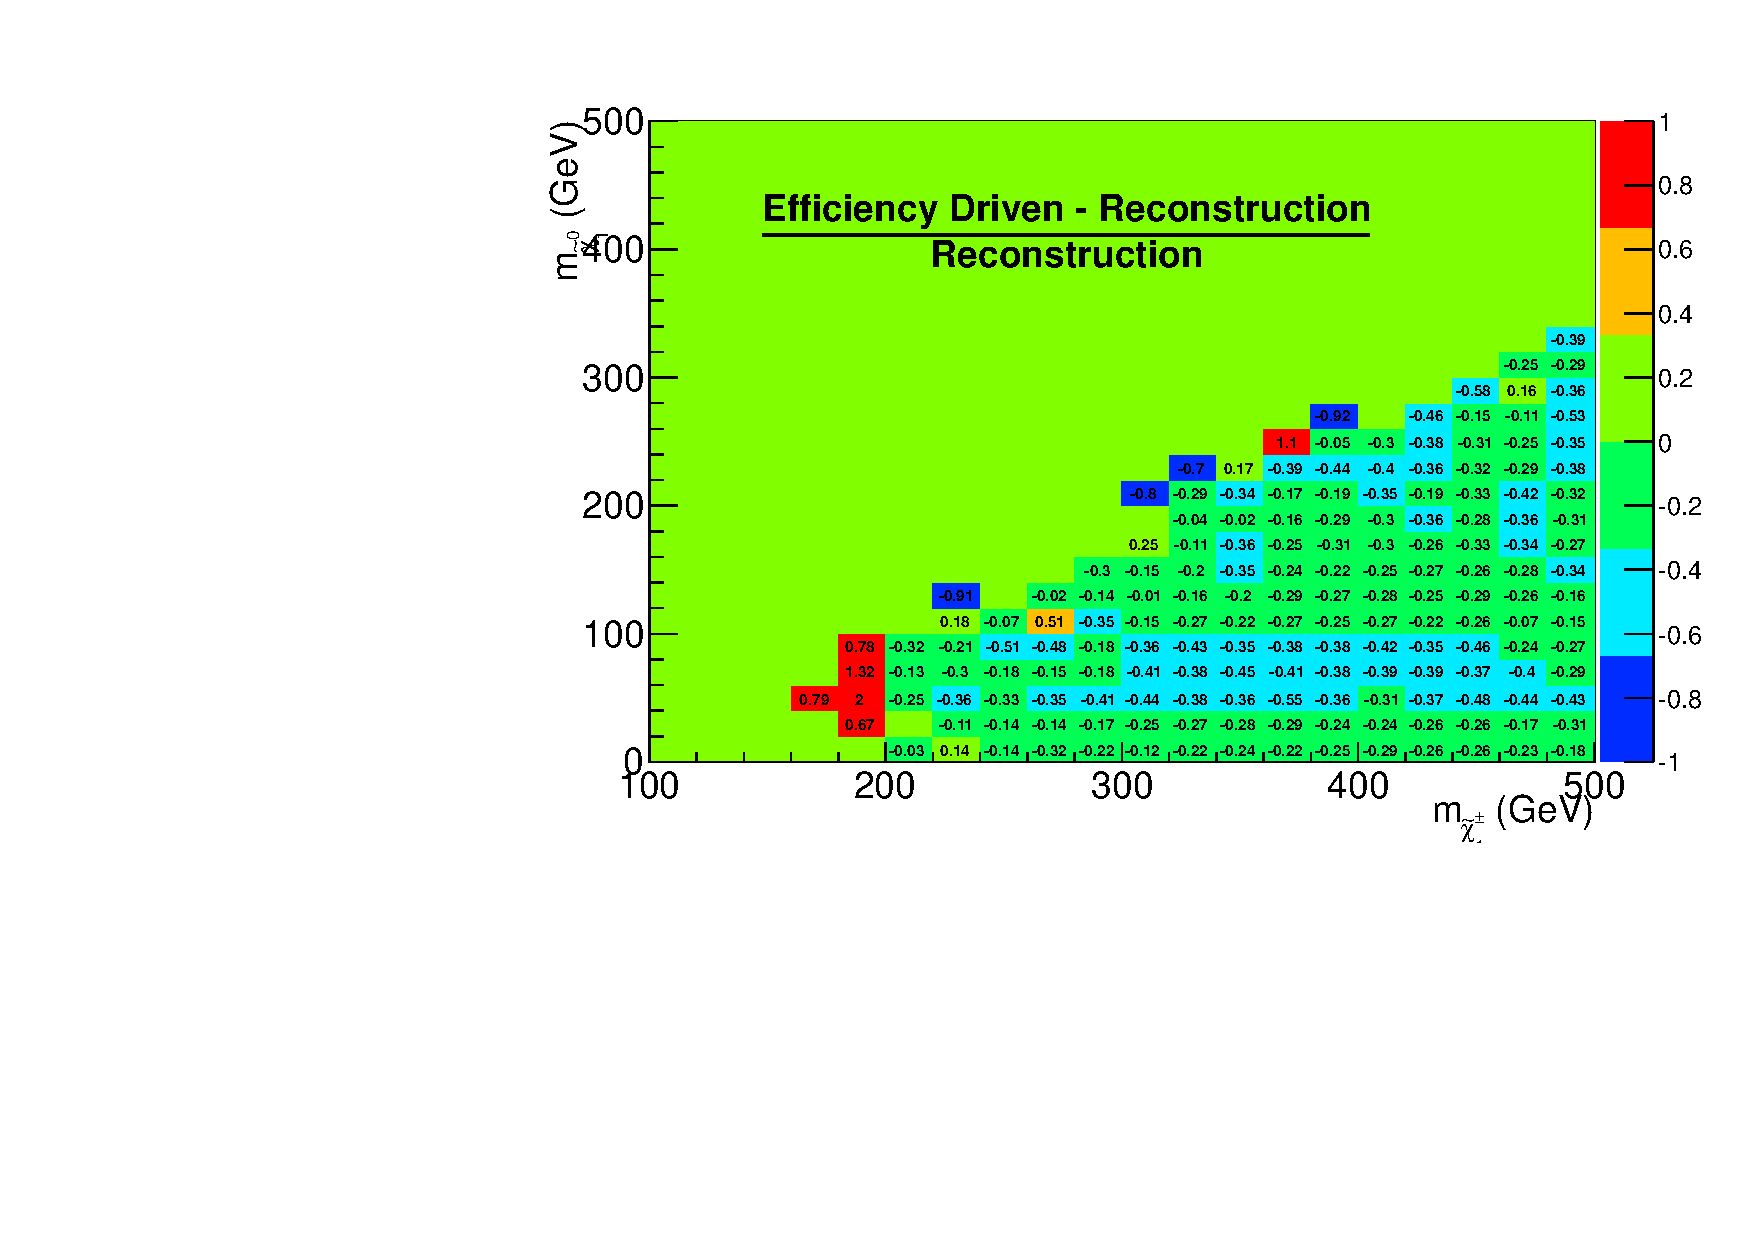
\includegraphics[width=0.5\textwidth,keepaspectratio=true]{ModelTesting/NormalizedDiffmuTau.pdf}
%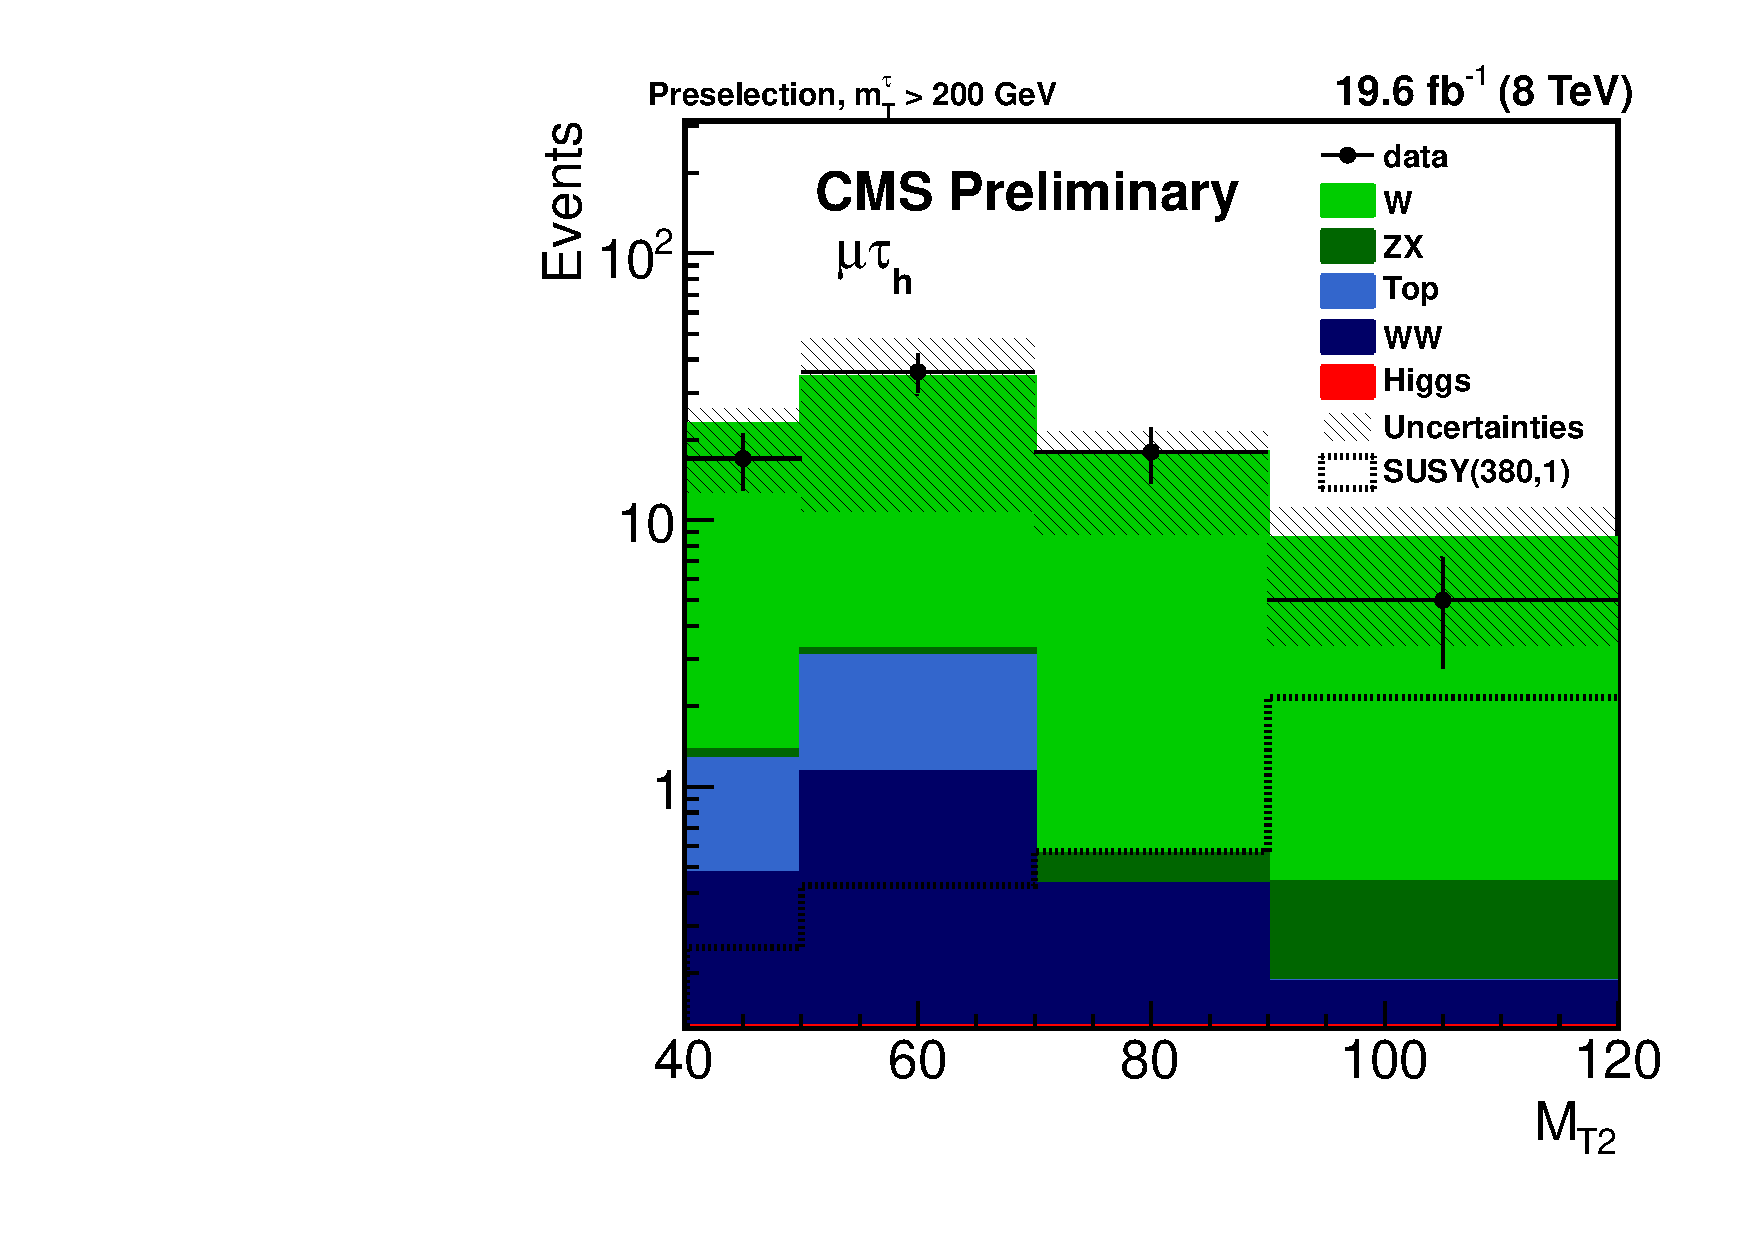
\includegraphics[width=0.475\textwidth,keepaspectratio=true]{StatisticsFig/MT2muTau_tauMTgt200_DDFake.pdf}
\caption{The relative difference between the results of the proposed method and the common analysis is shown for each SMS point. The results are shown for \muTau channel.}
\label{fig:NormalizedDiff}
\end{figure}
shows the relative difference of the yields driven by the
efficiencies and the yields from the full chain of simulation and reconstruction for each point of the SMS plane. The relative
difference is less than 30\% in the main part of the SMS plane.